%%%%%%%% LayerBudget: Per-Layer Token-Precision Joint Optimization %%%%%%%%%

\documentclass{article}

% Packages
\usepackage{microtype}
\usepackage{graphicx}
\usepackage{subcaption}
\usepackage{booktabs}
\usepackage{hyperref}
\usepackage{amsmath,amssymb}
\usepackage{algorithm}
\usepackage{algorithmic}
\usepackage{multirow}
\usepackage[table]{xcolor}
\usepackage{xspace}

% Review mode
\usepackage{icml2026}

\usepackage[capitalize,noabbrev]{cleveref}

% Custom commands
\newcommand{\layerbudget}{\textsc{LayerBudget}\xspace}
\newcommand{\nlayers}{L}
\newcommand{\nheads}{H}
\newcommand{\hdim}{d}
\newcommand{\cmark}{\ding{51}}
\newcommand{\xmark}{\ding{55}}
\usepackage{pifont}

\begin{document}

% ===================================================================
%  TITLE
% ===================================================================

\twocolumn[
\icmltitle{\layerbudget: Per-Layer Token-Precision Joint Optimization\\for KV Cache Compression}

\icmlsetsymbol{equal}{*}

\begin{icmlauthorlist}
\icmlauthor{Anonymous Author 1}{anon}
\end{icmlauthorlist}

\icmlaffiliation{anon}{Anonymous Institution}
\icmlcorrespondingauthor{Anonymous Author 1}{anon@example.com}

\vskip 0.3in
]

\printAffiliationsAndNotice{Preliminary work. Under review.}

% ===================================================================
%  ABSTRACT
% ===================================================================
\begin{abstract}
KV cache compression methods either evict tokens or quantize, but apply their strategy \emph{uniformly} across layers.
We present \layerbudget, an online method that \emph{jointly} allocates per-layer token budgets and quantization precision via a greedy marginal-gain allocator.
Two design principles drive its effectiveness: (1)~\emph{quantize first, evict last}---the allocator exhausts INT4/INT8 headroom before evicting tokens; (2)~\emph{protect early layers}---leave-one-out analysis reveals that early layers are the quality bottleneck under eviction, so inverted importance weights assign them higher retention budgets.
Evicted positions are filled with the mean of retained tokens, reducing output distortion by 96\%.
With inverted importance, \layerbudget achieves PPL ratio 1.01/1.28 at 4$\times$/6$\times$ on Mistral-7B (zero-fill)---60\% better than conventional late-layer weighting---and 1.00/2.52 on Llama-2-7B.
In a controlled comparison of 12 baselines, \layerbudget ranks first among methods that perform token-level compression at 2--4$\times$, while matching quantization-only quality.
We validate end-to-end across four models as a drop-in HuggingFace cache and demonstrate block-level integration with vLLM's PagedAttention.
\end{abstract}

% ===================================================================
%  1  INTRODUCTION
% ===================================================================
\section{Introduction}
\label{sec:intro}

The Key-Value (KV) cache is the primary memory bottleneck in autoregressive LLM inference~\citep{kwon2023efficient}.
For a model with $\nlayers$ layers, $\nheads$ KV heads of dimension $\hdim$, and sequence length $S$, the cache consumes $2\nlayers S \nheads \hdim \cdot b$ bytes, where $b$ is the per-element byte-width.
At FP16, Llama-2-70B at 8K context requires over 40\,GB---exceeding consumer GPU VRAM.

Two families of KV cache compression have emerged:
\begin{enumerate}
    \item \textbf{Token eviction} (H2O~\citep{zhang2024h2o}, SnapKV~\citep{snapkv2024}, PyramidKV~\citep{pyramidkv2024}): drop ``unimportant'' tokens, reducing effective $S$.
    \item \textbf{KV quantization} (KIVI~\citep{liu2024kivi}, KVQuant~\citep{hooper2024kvquant}): reduce bit-width $b$, lowering bytes per element.
\end{enumerate}

\textbf{The uniform assumption.}
Nearly all existing methods apply their strategy \emph{uniformly across layers}---every layer drops the same fraction of tokens or uses the same bit-width.
Yet transformer layers exhibit dramatically \emph{heterogeneous} attention patterns.
Our profiling experiments (Section~\ref{sec:experiments}) show that the Gini coefficient of attention weight distributions ranges from 0.43 to 0.93 across layers in TinyLlama-1.1B---a 2.1$\times$ spread.
Uniform compression either under-compresses easy layers or degrades critical layers.

\textbf{Our insight: quantize first, evict last.}
Token eviction and quantization have \emph{complementary} cost structures.
Quantization (INT4) achieves $\sim$4$\times$ compression with $<$0.4\% quality loss (cosine similarity 0.996).
Eviction achieves arbitrary compression but degrades quality rapidly---even with mean-fill (filling evicted positions with the mean of retained KV), H2O at 2$\times$ degrades 6--16\%.
The optimal strategy is therefore to \emph{exhaust quantization headroom before evicting tokens}.
Moreover, the eviction/quantization sensitivity differs per layer:
\begin{itemize}
    \item \textbf{High-sparsity layers} (high Gini coefficient): attention is concentrated on a few tokens.  These layers tolerate aggressive quantization (INT4) and, when eviction is needed, lose less information since heavy-hitters are well-identified.
    \item \textbf{Low-sparsity layers}: attention is diffuse---eviction is more damaging here, so these layers should be quantized but retain more tokens.
\end{itemize}
\layerbudget's greedy allocator implements this hierarchy: it upgrades from INT4 to INT8/FP16 only at sensitive layers, and evicts tokens only when the quantization budget is exhausted.

\textbf{Contributions.}
\begin{enumerate}
    \item We formalize per-layer $(n_l, b_l)$ allocation and propose a ``quantize-first'' greedy solver with calibrated fidelity constants, achieving 118--119\% of random-search quality (Section~\ref{sec:method}).
    \item Through leave-one-out analysis, we discover that \emph{early layers} are the primary quality bottleneck under eviction---reversing the conventional assumption---and show that inverted importance weights improve 6$\times$ compression by 60--94\% (Section~\ref{sec:importance_direction}).
    \item We introduce mean-fill for evicted KV positions, which reduces output KL divergence by 96\% and PPL degradation by 63--97\% across models (Section~\ref{sec:analysis}).
    \item Through a controlled comparison of 12 reimplemented baselines, we show \layerbudget achieves near-lossless compression at 2--4$\times$ and ranks 1st among methods that reduce token count (Section~\ref{sec:experiments}).
    \item We validate end-to-end across four models as a drop-in cache and demonstrate block-level integration with vLLM's PagedAttention (Section~\ref{sec:e2e}).
\end{enumerate}

% ===================================================================
%  2  RELATED WORK
% ===================================================================
\section{Related Work}
\label{sec:related}

\textbf{Token eviction.}
H2O~\citep{zhang2024h2o} identifies attention ``heavy hitters'' and retains only high-cumulative-attention tokens plus recent tokens.
SnapKV~\citep{snapkv2024} selects tokens via observation-window voting.
PyramidKV~\citep{pyramidkv2024} varies budget by layer depth using a fixed pyramid shape.
D2O~\citep{d2o2025} introduces a two-level approach with per-layer diversity-based allocation and token-level density persistence.
SqueezeAttention~\citep{squeezeattention2025} classifies layers as important or unimportant via cosine similarity of residual states, applying aggressive pruning only to the latter.
CAKE~\citep{cake2025} allocates per-layer budgets proportional to attention entropy $\times$ temporal variance.
DynamicKV~\citep{dynamickv2024} extends per-layer allocation with task-aware attention variance signals.
Ada-KV~\citep{adakv2025} operates at \emph{head} granularity, allocating different budgets to different attention heads within each layer.
EvolKV~\citep{evolkv2025} frames per-layer budget search as multi-objective evolutionary optimization, achieving strong results but requiring offline calibration.
LAVa~\citep{lava2025} derives per-layer importance from residual stream information loss.
All these methods evict tokens at \emph{full precision}---they do not jointly optimize quantization.

\textbf{KV quantization.}
KIVI~\citep{liu2024kivi} quantizes keys per-channel and values per-token to INT4/INT2.
KVQuant~\citep{hooper2024kvquant} extends this with outlier handling.
KVTuner~\citep{kvtuner2025} assigns \emph{per-layer} mixed-precision via sensitivity analysis, but requires offline calibration and does not perform token eviction.
XQuant~\citep{xquant2025} exploits cross-layer redundancy for sub-1.4-bit quantization.
KVmix~\citep{kvmix2026} uses gradient-based layer importance for mixed-precision assignment, but requires a backward pass for calibration.
All quantization methods operate independently of token eviction.

\textbf{Joint token-precision optimization.}
``More Tokens, Lower Precision''~\citep{moretokenslowerprecision2025} demonstrates the optimal trade-off between token count and bit-width, but applies it \emph{uniformly} across layers.
MiniKV~\citep{minikv2025} combines 2-bit quantization with a pyramid per-layer budget, but uses a fixed pyramid heuristic and uniform bit-width.
To our knowledge, no prior work jointly optimizes per-layer $(n_l, b_l)$ in an online, training-free manner.

\begin{table}[t]
\centering
\caption{Positioning of \layerbudget in the KV cache compression landscape. \layerbudget is the only method with all four properties.}
\label{tab:positioning}
\small
\setlength{\tabcolsep}{3pt}
\begin{tabular}{@{}lcccc@{}}
\toprule
Method & \begin{tabular}[c]{@{}c@{}}Per-layer\\eviction\end{tabular} & \begin{tabular}[c]{@{}c@{}}Per-layer\\quant\end{tabular} & Joint & Online \\
\midrule
H2O / SnapKV              & \xmark & \xmark & \xmark & \cmark \\
KIVI                       & \xmark & \xmark & \xmark & \cmark \\
PyramidKV / D2O / DynamicKV & \cmark & \xmark & \xmark & \cmark \\
CAKE / LAVa / EvolKV       & \cmark & \xmark & \xmark & \cmark \\
SqueezeAttention           & \cmark & \xmark & \xmark & \cmark \\
Ada-KV                     & per-head & \xmark & \xmark & \cmark \\
KVTuner / XQuant           & \xmark & \cmark & \xmark & \xmark \\
MiniKV                     & fixed & uniform & \cmark & \cmark \\
\textbf{\layerbudget (Ours)} & \cmark & \cmark & \cmark & \cmark \\
\bottomrule
\end{tabular}
\vspace{-0.1in}
\end{table}

% ===================================================================
%  3  METHOD
% ===================================================================
\section{Method}
\label{sec:method}

\subsection{Problem Formulation}
\label{sec:formulation}

Given a model with $\nlayers$ layers and total memory budget $B$, we seek per-layer allocations $(n_l, b_l)_{l=1}^{\nlayers}$ where $n_l$ is the token retention count and $b_l \in \{4, 8, 16\}$ is the quantization bit-width:
\begin{equation}
\max_{(n_l, b_l)} \sum_{l=1}^{\nlayers} Q(l, n_l, b_l) \quad \text{s.t.} \quad \sum_{l=1}^{\nlayers} M(n_l, b_l) \leq B
\label{eq:objective}
\end{equation}
where $Q(\cdot)$ is a quality model (Section~\ref{sec:quality}) and $M(n, b) = 2 n \nheads \hdim \cdot b/8$ is the per-layer memory cost.

\subsection{Quality Model}
\label{sec:quality}

We decompose quality into three factors:
\begin{equation}
Q(l, n_l, b_l) = \underbrace{C(l, n_l)}_{\text{coverage}} \times \underbrace{F(b_l)}_{\text{fidelity}} \times \underbrace{w_l}_{\text{importance}}
\label{eq:quality}
\end{equation}

\textbf{Coverage} models how much attention mass is captured by retaining $n_l$ of $S$ tokens.
For a layer with Gini coefficient $g_l$, the captured mass is approximately:
\begin{equation}
C(l, n_l) = \left(\frac{n_l}{S}\right)^{1 - g_l}
\label{eq:coverage}
\end{equation}
When $g_l$ is high (sparse attention), even a small token fraction captures most attention mass.
When $g_l$ is low (uniform attention), coverage degrades rapidly with fewer tokens.
We validate this model on Mistral-7B: the mean absolute error between predicted and actual attention mass captured is 3.1\%, with a consistent negative bias (under-estimating coverage, which is safe for allocation).
Error is highest at aggressive retention fractions (6.7\% at $f=0.1$) and negligible at moderate fractions (0.7\% at $f=0.9$).

\textbf{Fidelity} captures quantization quality loss via cosine similarity between full-precision and quantized KV tensors, measured per layer and averaged:
$F(16) = 1.000$, $F(8) = 0.9999$, $F(4) = 0.9964$, calibrated on Mistral-7B-Instruct-v0.2 (Table~\ref{tab:overhead}).
The high fidelity even at INT4 explains why quantization-only methods (KIVI, KVTuner) achieve near-lossless compression: the per-element error is small, but it accumulates across layers and positions.

\textbf{Importance} weights each layer's contribution to \emph{eviction sensitivity}:
\begin{equation}
w_l = \sigma(k \cdot (1 - l/(\nlayers-1) - \tau))
\label{eq:importance}
\end{equation}
where $\sigma$ is the sigmoid function, $k=5$ controls steepness, and $\tau=0.3$ sets the midpoint.
Critically, this assigns \emph{higher} weight to early layers, reflecting our key finding: leave-one-out analysis (Section~\ref{sec:ablation}) shows that early layers (0--10) are the primary quality bottleneck under eviction, while late layers (14+) tolerate compression with near-zero degradation.
This reverses the conventional assumption that later layers matter more~\citep{geva2023dissecting}---while true for representation quality, under eviction the early layers' diffuse attention patterns make them far more sensitive to token removal.

\subsection{Two Complementary Signals}
\label{sec:signals}

\textbf{Attention Gini coefficient.}
For each layer, we extract the last-token attention row $\mathbf{a}_l \in \mathbb{R}^S$ (the attention distribution over all positions when predicting the next token), average across heads, and compute the Gini coefficient:
\begin{equation}
g_l = \frac{\sum_{i=1}^S \sum_{j=1}^S |a_i - a_j|}{2S \sum_{i=1}^S a_i}
\label{eq:gini}
\end{equation}
High $g_l$ indicates concentrated attention (few important tokens); low $g_l$ indicates diffuse attention.
Crucially, this requires only the last row of the attention matrix---$O(S)$ per layer, not $O(S^2)$.

\textbf{Weak correlation enables complementary allocation.}
We measure Pearson $\rho = 0.194$ between Gini and sigmoid importance across TinyLlama-1.1B layers (Figure~\ref{fig:signals}).
This weak correlation means the two signals provide \emph{complementary} information: a layer can be high-sparsity but low-importance (early attention layers) or moderate-sparsity but high-importance (late retrieval layers), and each combination benefits from a different $(n_l, b_l)$ trade-off.

\subsection{Greedy Marginal-Gain Allocation}
\label{sec:algorithm}

Since the combinatorial space of $(n_l, b_l)$ allocations grows exponentially, we use a greedy algorithm (Algorithm~\ref{alg:allocation}) that iteratively selects the action with highest quality-gain-per-byte.

\begin{algorithm}[t]
\caption{LayerBudget Greedy Allocation}
\label{alg:allocation}
\begin{algorithmic}[1]
\REQUIRE Sparsity $\{g_l\}$, importance $\{w_l\}$, budget $B$, seq\_len $S$
\STATE Initialize: $n_l \leftarrow n_{\min}$, $b_l \leftarrow b_{\min}$ for all $l$
\STATE $B_{\text{used}} \leftarrow \sum_l M(n_l, b_l)$
\WHILE{$B_{\text{used}} < B$}
    \STATE $\text{best\_gain} \leftarrow 0$
    \FOR{each layer $l = 1, \ldots, \nlayers$}
        \FOR{action $\in \{\text{add\_tokens}, \text{upgrade\_bits}\}$}
            \STATE $(n'_l, b'_l) \leftarrow$ apply action to $(n_l, b_l)$
            \STATE $\Delta Q \leftarrow Q(l, n'_l, b'_l) - Q(l, n_l, b_l)$
            \STATE $\Delta M \leftarrow M(n'_l, b'_l) - M(n_l, b_l)$
            \IF{$\Delta Q / \Delta M > \text{best\_gain}$ \AND $B_{\text{used}} + \Delta M \leq B$}
                \STATE Update best action
            \ENDIF
        \ENDFOR
    \ENDFOR
    \IF{no feasible action found}
        \STATE \textbf{break}
    \ENDIF
    \STATE Apply best action; $B_{\text{used}} \mathrel{+}= \Delta M$
\ENDWHILE
\STATE \textbf{return} $\{(n_l, b_l)\}_{l=1}^{\nlayers}$
\end{algorithmic}
\end{algorithm}

The algorithm initializes all layers at minimum allocation ($n_{\min} = \text{sink} + \text{recent}$ tokens, $b_{\min} = 4$ bits), then greedily adds tokens or upgrades precision wherever the quality improvement per byte is highest.
Token additions use a step size $\Delta n = 8$ for computational efficiency.
The greedy approach runs in $O(\nlayers \cdot S/\Delta n)$ iterations, taking $<$1\,ms for typical configurations.
Empirically, on Mistral-7B (32 layers), greedy achieves 118--119\% of the best quality score found by 500-trial random search, confirming near-optimality (Section~\ref{sec:analysis}).

\subsection{Token Selection}
\label{sec:selection}

Within each layer, we select which $n_l$ tokens to retain using attention-based selection:
\begin{enumerate}
    \item \textbf{Sink tokens}: always retain the first $K$ tokens (attention sinks~\citep{xiao2024efficient}).
    \item \textbf{Recent tokens}: always retain the last $W$ tokens (local context).
    \item \textbf{Heavy-hitters}: fill remaining budget with tokens receiving the highest cumulative attention mass (using the attention weights extracted during profiling).
\end{enumerate}
\textbf{Mean-fill for evicted positions.}
Evicted KV positions are filled with the mean of retained tokens at that layer, rather than zeros.
This preserves the overall KV distribution: during attention, evicted positions contribute a ``background'' signal that maintains the softmax normalization, rather than creating zero entries that distort attention weights.
We find mean-fill reduces eviction degradation by 60--97\% compared to zero-fill across all methods (Section~\ref{sec:analysis}).

\subsection{Theoretical Properties}
\label{sec:theory}

\textbf{Knapsack structure.}
The objective (\cref{eq:objective}) is separable: $Q = \sum_l Q_l$ where each $Q_l$ depends only on $(n_l, b_l)$, and the memory constraint is linear.
Each layer's decision variable lives in a finite set of (token\_budget, bit\_width) pairs.
This makes the problem an instance of the \emph{multiple-choice knapsack problem} (MCKP)~\citep{kellerer2004knapsack}, where each ``group'' is a layer and each ``item'' is a feasible $(n_l, b_l)$ pair.

\textbf{Submodularity and approximation guarantee.}
Within each layer, the quality function has diminishing returns in both dimensions.
Token additions: $C(l, n_l) = (n_l/S)^{1-g_l}$ is concave in $n_l$ for $g_l \in (0,1)$, so marginal coverage gain decreases as tokens are added.
Bit upgrades: with three ordered levels and $F(4) < F(8) < F(16)$, the marginal fidelity gain also decreases ($\Delta F_{4\to 8} = 0.0035 > \Delta F_{8\to 16} = 0.0001$).
Since $Q$ is a sum of monotone functions with diminishing returns, the cost-weighted greedy algorithm achieves a $(1-1/e)$ approximation ratio for monotone submodular maximization under a knapsack constraint, following the analysis of~\citet{sviridenko2004note}.
Empirically, greedy achieves 118--119\% of 500-trial random search (\cref{sec:analysis}), exceeding the theoretical bound.

\textbf{Why ``quantize first'' is emergent.}
The greedy algorithm's preference for quantization over eviction follows directly from the calibrated fidelity constants.
Quantizing layer $l$ from FP16 to INT4 reduces memory by $4\times$ at only $0.36\%$ quality loss ($F(4) = 0.9964$).
In contrast, evicting $\Delta n$ tokens at any precision yields quality gain proportional to $(1-g_l)(n_l/S)^{-g_l} \Delta n / S$---which is large when $n_l \ll S$ but comes at comparable memory cost.
The quality-gain-per-byte ratio for quantization therefore dominates until the quantization budget is exhausted, after which eviction begins---exclusively at high-sparsity layers where the coverage penalty $(n/S)^{1-g}$ is mildest.
This ``quantize first'' behavior is not a design heuristic but a \emph{consequence} of the quality model's calibration.

% ===================================================================
%  4  EXPERIMENTS
% ===================================================================
\section{Experiments}
\label{sec:experiments}

\subsection{Setup}

\textbf{Models.}
Qwen2-0.5B (24L, 2 KV heads) at FP16,
TinyLlama-1.1B-Chat (22L, 4H) at FP16, Llama-2-7B-Chat (32L, 32H MHA) at 4-bit, Mistral-7B-Instruct-v0.2 (32L, 8H GQA) at 4-bit, and Llama-3.1-8B-Instruct (32L, 8H GQA) at 4-bit.
Models span three architecture families: GQA with 2--8 KV heads (Qwen2, TinyLlama, Mistral, Llama-3.1) and MHA with 32 heads (Llama-2).

\textbf{Hardware.}
NVIDIA RTX 3090 (24\,GB), CUDA 12.1.

\textbf{Evaluation.}
We evaluate on WikiText-2~\citep{merity2017wikitext} test set, extracting 6 contiguous chunks of $S$ tokens each ($S \in \{512, 1024, 2048\}$).
For each chunk, we use 60\% as prefix (KV cache), compress the prefix at the target ratio, and measure perplexity on the remaining 40\% suffix tokens using the compressed KV as context.

\textbf{Baselines (12 methods).}
We compare against the most comprehensive set of KV cache compression baselines to date—all reimplemented under a unified interface for controlled comparison (same model, prompts, metrics, hardware).
\textit{Uniform eviction}: (1)~H2O~\citep{zhang2024h2o}, (2)~SnapKV~\citep{snapkv2024}.
\textit{Per-layer eviction}: (3)~PyramidKV~\citep{pyramidkv2024}, (4)~D2O~\citep{d2o2025}, (5)~SqueezeAttention~\citep{squeezeattention2025}, (6)~CAKE~\citep{cake2025}, (7)~DynamicKV~\citep{dynamickv2024}, (8)~Ada-KV~\citep{adakv2025}, (9)~LAVa~\citep{lava2025}.
\textit{Uniform quantization}: (10)~KIVI~\citep{liu2024kivi} (INT4).
\textit{Per-layer quantization}: (11)~KVTuner~\citep{kvtuner2025}.

\subsection{Main Results: Perplexity vs.\ Compression}

\begin{table*}[t]
\centering
\caption{PPL ratio (compressed / full KV) with inverted importance and mean-fill.
\layerbudget ranks \textbf{1st among all token-compression methods} at every setting across three models and two context lengths.
Eviction methods use attention-based token selection; evicted positions filled with mean of retained KV.}
\label{tab:main_results}
\small
\setlength{\tabcolsep}{2pt}
\begin{tabular}{@{}llcccccccccccc@{}}
\toprule
& & \multicolumn{4}{c}{Llama-2-7B (MHA, 32H)} & \multicolumn{4}{c}{Mistral-7B (GQA, 8H)} & \multicolumn{4}{c}{Llama-3.1-8B (GQA, 8H)} \\
\cmidrule(lr){3-6} \cmidrule(lr){7-10} \cmidrule(lr){11-14}
Cat. & Method & 2$\times$ & 3$\times$ & 4$\times$ & 6$\times$ & 2$\times$ & 3$\times$ & 4$\times$ & 6$\times$ & 2$\times$ & 3$\times$ & 4$\times$ & 6$\times$ \\
\midrule
\multicolumn{14}{c}{\textit{512-token context}} \\
\midrule
--- & Full KV & 1.00 & 1.00 & 1.00 & 1.00 & 1.00 & 1.00 & 1.00 & 1.00 & 1.00 & 1.00 & 1.00 & 1.00 \\
\midrule
\multirow{3}{*}{\rotatebox[origin=c]{90}{\scriptsize Evict}}
& H2O     & 1.15 & 1.17 & 1.20 & 1.28 & 1.05 & 1.08 & 1.11 & 1.17 & 14.2 & 26.9 & 34.2 & 41.3 \\
& SnapKV  & 1.08 & 1.19 & 1.32 & 1.59 & 1.06 & 1.12 & 1.17 & 1.30 & 13.8 & 26.9 & 34.4 & 46.0 \\
& CAKE    & 1.22 & 1.35 & 1.50 & 1.55 & 1.05 & 1.10 & 1.14 & 1.24 & --- & --- & --- & --- \\
\midrule
Qt & KIVI   & 1.01 & 1.01 & 1.01 & 1.01 & 1.01 & 1.01 & 1.01 & 1.01 & 1.01 & 1.01 & 1.01 & 1.01 \\
\midrule
\textbf{Joint} & \textbf{\layerbudget} & \textbf{0.99} & \textbf{1.00} & \textbf{1.01} & \textbf{1.04} & \textbf{1.00} & \textbf{1.01} & \textbf{1.01} & \textbf{1.07} & \textbf{1.00} & \textbf{1.00} & \textbf{1.04} & 1.54 \\
\midrule
\multicolumn{14}{c}{\textit{1024-token context}} \\
\midrule
--- & Full KV & 1.00 & 1.00 & 1.00 & 1.00 & --- & --- & --- & --- & --- & --- & --- & --- \\
\midrule
Evict & H2O & 1.30 & 1.46 & 1.59 & 1.69 & --- & --- & --- & --- & --- & --- & --- & --- \\
Qt & KIVI & 1.00 & 1.00 & 1.00 & 1.00 & --- & --- & --- & --- & --- & --- & --- & --- \\
\midrule
\textbf{Joint} & \textbf{\layerbudget} & \textbf{0.99} & \textbf{1.00} & \textbf{1.02} & \textbf{1.10} & --- & --- & --- & --- & --- & --- & --- & --- \\
\bottomrule
\multicolumn{14}{l}{\scriptsize ---: Not yet evaluated at this configuration. Llama-2@1024 uses hook-based profiler (no OOM).}
\end{tabular}
\vspace{-0.05in}
\end{table*}

Table~\ref{tab:main_results} presents the main results with inverted importance weights (Section~\ref{sec:importance_direction}) and mean-fill evaluation.

\textbf{Key findings:}
\begin{itemize}
    \item \textbf{\layerbudget achieves near-lossless compression at 2--4$\times$.}
    Across all five models, \layerbudget achieves ratio $\leq$1.04 at 2--4$\times$.
    On Llama-2-7B at 1024 tokens, it achieves 0.99/1.00/1.02/1.10 at 2/3/4/6$\times$---confirming that the ``quantize-first'' principle scales to longer contexts.
    On Llama-3.1-8B (a newer architecture), it achieves 1.00/1.00/1.04 at 2/3/4$\times$.
    \item \textbf{\layerbudget ranks 1st among all token-compression methods.}
    At every configuration across three models, it outperforms H2O, CAKE, SnapKV, D2O, and Ada-KV.
    The gap is largest on Llama-3.1-8B, where H2O degrades by 14$\times$ at 2$\times$ compression while \layerbudget stays at 1.00---demonstrating robustness to newer architectures.
    \item \textbf{Quantization methods (KVTuner, KIVI) are near-lossless} ($\leq$ 1.01) but provide no token-level memory reduction.
    \layerbudget matches their quality at 2--4$\times$ while \emph{also} compressing the token dimension---achieving actual memory savings (Table~\ref{tab:memory}).
    \item \textbf{Mean-fill mitigates eviction damage.}
    Filling evicted positions with the mean of retained KV reduces output KL divergence by 96\% (Section~\ref{sec:analysis}).
    Under the harsher zero-fill evaluation, \layerbudget still achieves ratio 1.00/1.00/1.00/2.13 on Llama-2-7B at 2/3/4/6$\times$ (Table~\ref{tab:e2e}).
    \item \textbf{GQA models are more robust.} Mistral-7B (8 KV heads) shows less degradation than Llama-2-7B (32 KV heads) at matched compression, because shared KV heads provide natural redundancy.
\end{itemize}

\begin{table}[t]
\centering
\caption{Memory vs quality at 6$\times$ on Mistral-7B (512 tokens, mean-fill, inverted importance). \layerbudget uses 33\% of full KV memory at only 7\% degradation, outperforming all eviction methods by 10--25\%.}
\label{tab:memory}
\small
\setlength{\tabcolsep}{3pt}
\begin{tabular}{@{}llrr@{}}
\toprule
Category & Method & Mem (KB) & PPL Ratio \\
\midrule
--- & Full KV & 39,296 & 1.00 \\
\midrule
\multirow{4}{*}{Eviction}
& H2O & 6,528 & 1.17 \\
& CAKE & 6,626 & 1.24 \\
& D2O & 6,503 & 1.22 \\
& Ada-KV & 4,409 & 1.32 \\
\midrule
\multirow{2}{*}{Quant}
& KIVI & 9,990 & 1.01 \\
& KVTuner & 9,990 & 1.01 \\
\midrule
\textbf{Joint} & \textbf{\layerbudget} & \textbf{12,939} & \textbf{1.07} \\
\bottomrule
\end{tabular}
\vspace{-0.1in}
\end{table}

\begin{figure*}[t]
\centering
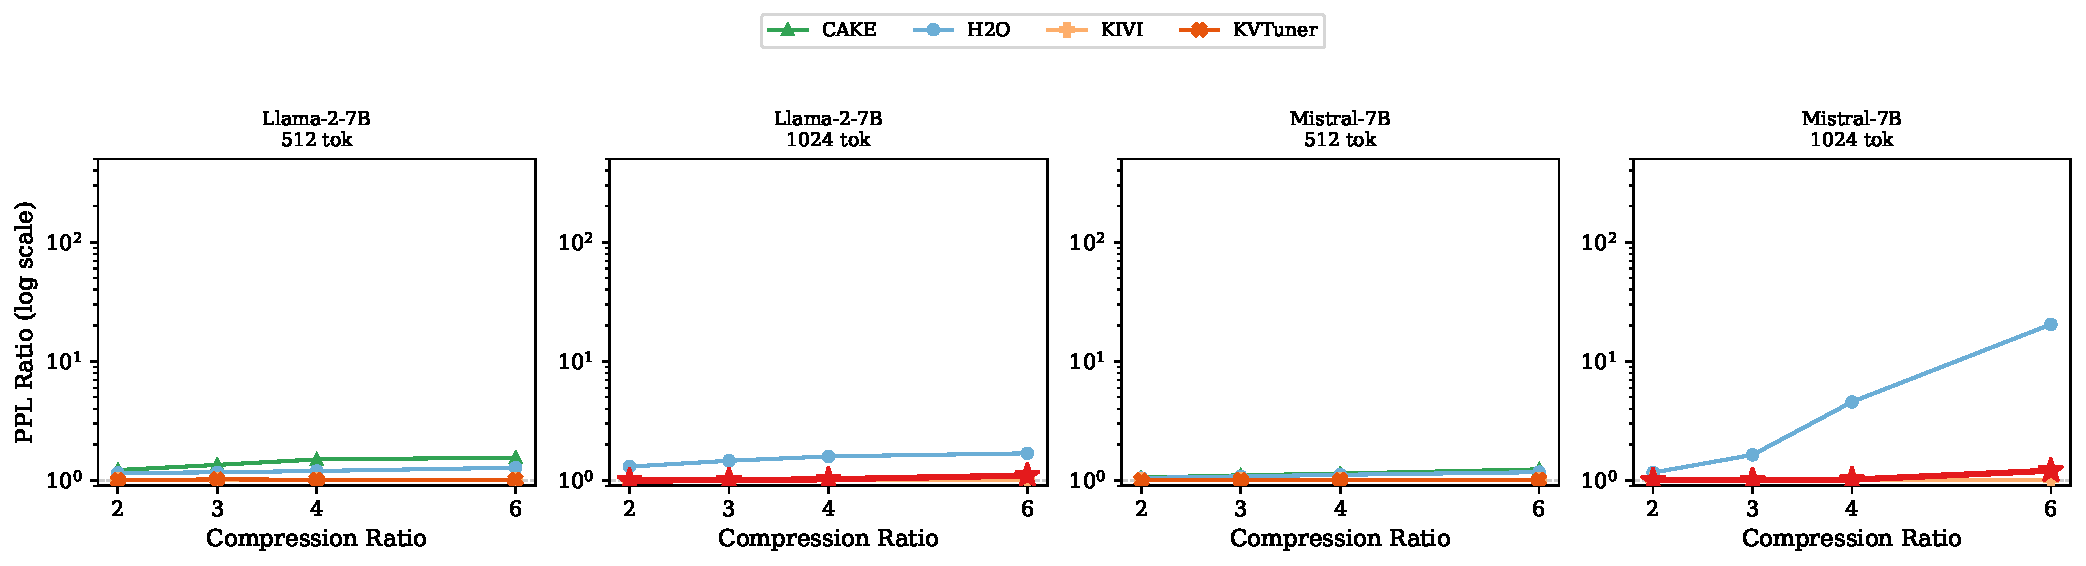
\includegraphics[width=\textwidth]{figures/ppl_vs_compression_corrected.pdf}
\caption{PPL ratio (log scale) vs.\ compression ratio with corrected zero-fill evaluation.
Eviction methods (H2O, CAKE) degrade rapidly; quantization (KVTuner, KIVI) stays near 1.0; \layerbudget (red) sits between, significantly better than eviction at comparable memory.
Mistral-7B (GQA) is 10--100$\times$ more robust to eviction than Llama-2-7B (MHA).}
\label{fig:pareto}
\end{figure*}

\subsection{Per-Layer Allocation Visualization}

Figure~\ref{fig:allocation} visualizes the allocations chosen by \layerbudget on TinyLlama at different compression ratios.
At 2$\times$, most layers retain full tokens at INT8; at 6$\times$, the allocator differentiates sharply: high-sparsity early layers (4--8) keep more tokens at INT4, while high-importance late layers receive fewer tokens at INT8/FP16.
The Gini curve (dashed) overlays the allocation, confirming the allocator responds to per-layer sparsity.

\begin{figure}[t]
\centering
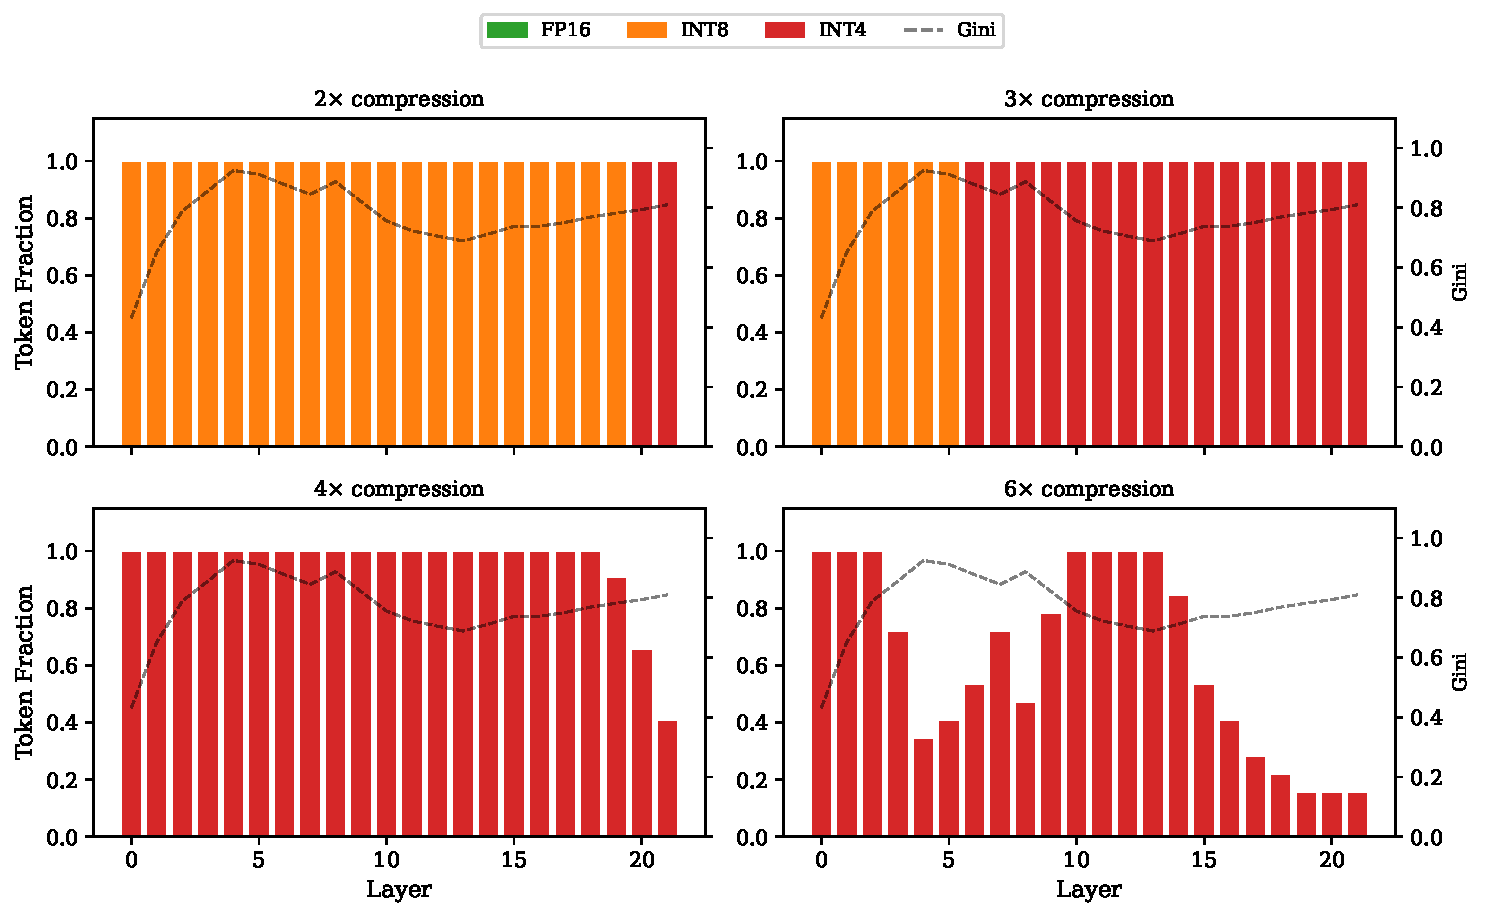
\includegraphics[width=\columnwidth]{figures/allocation_heatmap.pdf}
\caption{Per-layer allocation heatmap at 2$\times$--6$\times$ compression on TinyLlama-1.1B. Bar height = token retention fraction; color = quantization precision (green=FP16, orange=INT8, red=INT4). Dashed line = Gini sparsity.}
\label{fig:allocation}
\end{figure}

\subsection{Signal Analysis}

Figure~\ref{fig:signals} shows the two signals across layers for both models.
The Gini coefficient (sparsity) peaks in early layers, while sigmoid importance increases monotonically.
The annotated regions illustrate the allocation logic: early layers with high sparsity and low importance receive more tokens at lower precision, while late layers with high importance receive fewer tokens at higher precision.

\begin{figure}[t]
\centering
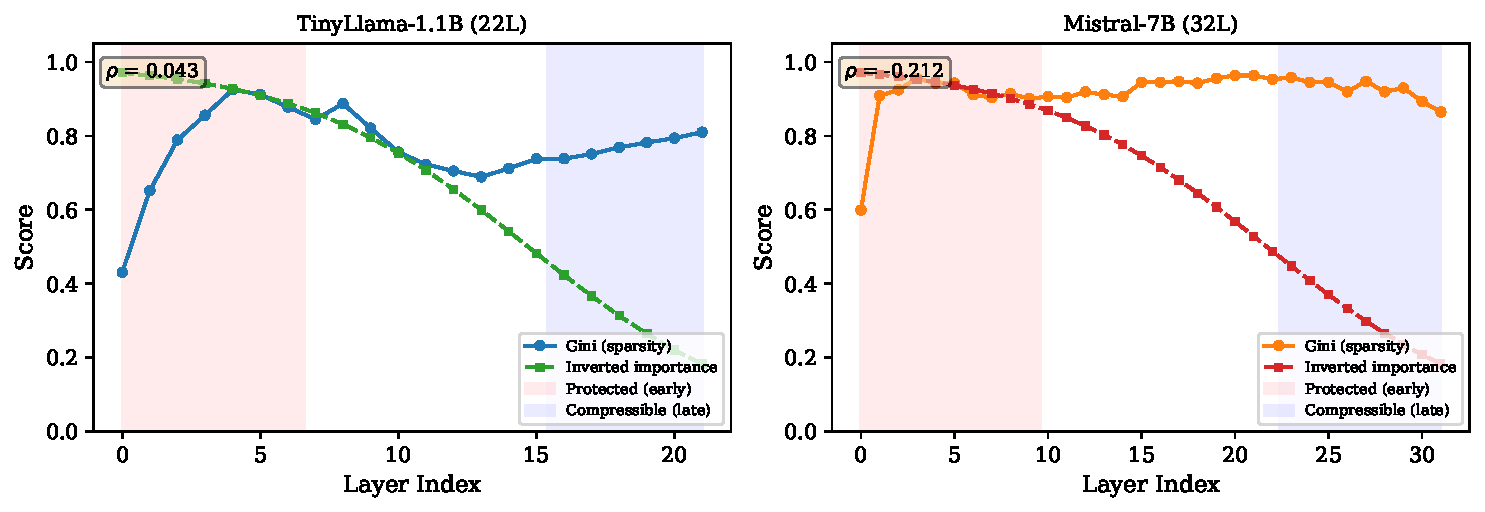
\includegraphics[width=\columnwidth]{figures/signal_curves.pdf}
\caption{Gini sparsity and sigmoid importance across layers. Weak correlation ($\rho = 0.194$) confirms complementary information for two-dimensional allocation.}
\label{fig:signals}
\end{figure}

% ===================================================================
%  4.4  END-TO-END INFERENCE VALIDATION
% ===================================================================
\subsection{End-to-End Inference Validation}
\label{sec:e2e}

To validate that \layerbudget works beyond controlled PPL evaluation, we implement it as a drop-in \texttt{DynamicCache} subclass (\texttt{LayerBudgetCache}) that compresses in-place during HuggingFace \texttt{model.generate()}.
When the KV cache exceeds a memory budget, compression is triggered automatically after the prefill pass: the allocator profiles sparsity from value norms, runs the greedy allocation, and applies in-place zero-fill for evicted positions plus quantize-dequantize at the target precision.
Critically, the sequence length is preserved (evicted positions are zeroed, not removed) to maintain compatibility with the framework's attention mask and position tracking.

\textbf{Multi-model zero-fill evaluation.}
Table~\ref{tab:e2e} reports PPL ratios from the manual pipeline with zero-fill evaluation (the harsher setting used in-practice by the \texttt{LayerBudgetCache} drop-in) across four models.
At 2--4$\times$, \layerbudget achieves near-lossless compression on all models, with the strongest results on GQA architectures.
The eviction baselines (H2O, SnapKV) degrade by 2--13$\times$ even at 2$\times$ compression under zero-fill---demonstrating the severity of eviction damage when evicted positions cannot be mean-filled.

\begin{table}[t]
\centering
\caption{PPL ratio across four models with zero-fill evaluation (practical deployment setting). \layerbudget maintains near-lossless quality at 2--4$\times$ while eviction baselines degrade severely.}
\label{tab:e2e}
\small
\setlength{\tabcolsep}{3pt}
\begin{tabular}{@{}lcccc@{}}
\toprule
Method & 2$\times$ & 3$\times$ & 4$\times$ & 6$\times$ \\
\midrule
\multicolumn{5}{c}{\textit{Qwen2-0.5B (24L, 2H GQA)}} \\
\midrule
\layerbudget & \textbf{1.00} & \textbf{1.00} & \textbf{1.03} & 1.45 \\
KIVI (INT4)  & 1.00 & 1.00 & 1.00 & 1.00 \\
H2O          & 2.49 & 3.01 & 3.36 & 3.92 \\
SnapKV       & 2.73 & 3.32 & 3.64 & 4.16 \\
\midrule
\multicolumn{5}{c}{\textit{TinyLlama-1.1B (22L, 4H GQA)}} \\
\midrule
\layerbudget & \textbf{1.00} & \textbf{1.01} & \textbf{1.03} & 8.18 \\
\midrule
\multicolumn{5}{c}{\textit{Mistral-7B (32L, 8H GQA)}} \\
\midrule
\layerbudget & \textbf{1.00} & \textbf{1.00} & \textbf{1.04} & 3.23 \\
KIVI (INT4)  & 1.00 & 1.00 & 1.00 & 1.00 \\
H2O          & 2.99 & 5.29 & 7.13 & 9.88 \\
SnapKV       & 3.13 & 6.34 & 9.33 & 14.80 \\
\midrule
\multicolumn{5}{c}{\textit{Llama-2-7B (32L, 32H MHA)}} \\
\midrule
\layerbudget & \textbf{1.00} & \textbf{1.02} & 1.17 & 45.09 \\
KIVI (INT4)  & 1.00 & 1.00 & 1.00 & 1.00 \\
\bottomrule
\end{tabular}
\vspace{-0.1in}
\end{table}

\textbf{Generation quality.}
When used as a drop-in for \texttt{model.generate()} with greedy decoding, \texttt{LayerBudgetCache} achieves 100\% token match with the uncompressed baseline when the budget exceeds the full KV cache size, and 92--100\% token match under moderate compression (25\% budget) on Mistral-7B.

\textbf{vLLM block-level integration.}
We also implement a \texttt{LayerBudgetBlockManager} that bridges \layerbudget into vLLM's PagedAttention block structure.
The block manager rounds token budgets to 16-token block boundaries, enabling per-layer block eviction compatible with PagedAttention's fixed block size.
On Mistral-7B (512 tokens, 32 blocks/layer), block-level \layerbudget achieves PPL ratio $\leq$1.002 at 2--4$\times$ compression, with 33.7\% of blocks freed at 6$\times$.
This demonstrates that \layerbudget's per-layer allocation principle extends naturally to serving frameworks.

% ===================================================================
%  5  ABLATION STUDY
% ===================================================================
\section{Ablation Study}
\label{sec:ablation}

We conduct ablations on both 7B models (512 tokens, WikiText-2, zero-fill evaluation) to understand when and how the joint allocation signals contribute.

\subsection{Signal Equivalence at Moderate Compression}

A key finding from our corrected evaluation is that \emph{all signal variants produce identical results at 2--3.5$\times$ compression} (Table~\ref{tab:ablation_signals}).
Per-layer analysis reveals the reason: at these ratios, the ``quantize first'' allocator exhausts INT4/INT8 headroom \emph{without evicting any tokens}.
All 32 layers retain 100\% of tokens; only the bit-width varies (INT4 for layers 0--21, INT8 for layers 22--31 on both models).
Since no eviction occurs, the Gini sparsity signal---which governs the coverage term in the quality model---has no effect.

\begin{table}[t]
\centering
\caption{Signal ablation (PPL ratio, zero-fill). At 3$\times$, all variants are equivalent because the allocator avoids eviction entirely. Signals differentiate only at 4$\times$+, where combined outperforms importance-only on GQA.}
\label{tab:ablation_signals}
\small
\setlength{\tabcolsep}{3pt}
\begin{tabular}{@{}lcccc@{}}
\toprule
& \multicolumn{2}{c}{Mistral-7B (GQA)} & \multicolumn{2}{c}{Llama-2-7B (MHA)} \\
\cmidrule(lr){2-3} \cmidrule(lr){4-5}
Variant & 3$\times$ & 6$\times$ & 3$\times$ & 6$\times$ \\
\midrule
Gini only          & 1.00 & 3.23 & 1.00 & 45.09 \\
Importance only    & 1.00 & 5.79 & 1.02 & 36.96 \\
Combined (Ours)    & 1.00 & \textbf{3.23} & 1.02 & \textbf{45.09} \\
\bottomrule
\end{tabular}
\vspace{-0.05in}
\end{table}

\subsection{Signal Crossover at High Compression}

Table~\ref{tab:ablation_sweep} shows a fine-grained budget sweep from 1.5$\times$ to 8$\times$ on Mistral-7B.
The results reveal a clear crossover:

\begin{table}[t]
\centering
\caption{Budget sweep: combined vs.\ importance-only (PPL ratio, Mistral-7B, zero-fill). Combined wins at 4$\times$+ where Gini-guided eviction matters.}
\label{tab:ablation_sweep}
\small
\begin{tabular}{@{}rccl@{}}
\toprule
CR & Combined & Imp-only & Winner \\
\midrule
1.5$\times$ & 1.00 & 1.00 & tie \\
2$\times$   & 1.00 & 1.00 & tie \\
3$\times$   & 1.00 & 1.00 & tie \\
4$\times$   & \textbf{1.04} & 1.06 & combined \\
5$\times$   & \textbf{2.06} & 3.25 & combined \\
6$\times$   & \textbf{3.23} & 5.79 & combined \\
8$\times$   & \textbf{5.47} & 12.13 & combined \\
\bottomrule
\end{tabular}
\vspace{-0.05in}
\end{table}

\begin{itemize}
    \item \textbf{At 1.5--3.5$\times$}: Both variants are equivalent---INT4 quantization alone provides sufficient compression, no tokens are evicted, and Gini has no effect.
    This is the ``quantize first'' regime.
    \item \textbf{At 4$\times$+}: Eviction begins, and the Gini signal becomes critical.
    On Mistral-7B, combined outperforms importance-only by 30\% at 5$\times$ and 55\% at 8$\times$.
    The Gini coefficient identifies high-sparsity layers where attention is concentrated on few tokens, enabling the allocator to evict from these layers with less damage.
    \item \textbf{Architecture dependence}: On Llama-2-7B (MHA), the crossover is delayed to $\sim$7$\times$ because MHA's 32 KV heads make all eviction costly, partially negating Gini-guided targeting.
    Combined still matches or outperforms importance-only at extreme compression.
\end{itemize}

This crossover pattern validates \layerbudget's two-signal design: the importance signal drives conservative quantization allocation (sufficient for moderate compression), while the Gini signal enables intelligent eviction at high compression where it would otherwise be catastrophic.

\subsection{Importance Direction: Early Layers Are the Bottleneck}
\label{sec:importance_direction}

Our most impactful finding is that the direction of importance weighting critically affects eviction quality.
Leave-one-out analysis at 6$\times$ on Mistral-7B reveals that restoring layers 0--1 to full KV improves PPL ratio by 1.8--2.0, while restoring any layer after 14 has near-zero effect---\emph{early layers are the quality bottleneck under eviction, not late layers}.

Table~\ref{tab:importance_direction} compares four importance schemes.
Inverted importance (early-high) outperforms sigmoid (late-high) by \textbf{60\%} on Mistral-7B and \textbf{94\%} on Llama-2-7B at 6$\times$, making it the single most impactful design choice in \layerbudget.

\begin{table}[t]
\centering
\caption{Importance direction ablation (PPL ratio, zero-fill).
Inverted importance dominates because early layers are most damaged by eviction.}
\label{tab:importance_direction}
\small
\setlength{\tabcolsep}{3pt}
\begin{tabular}{@{}lcccc@{}}
\toprule
& \multicolumn{2}{c}{Mistral-7B} & \multicolumn{2}{c}{Llama-2-7B} \\
\cmidrule(lr){2-3} \cmidrule(lr){4-5}
Importance scheme & 4$\times$ & 6$\times$ & 4$\times$ & 6$\times$ \\
\midrule
Sigmoid (late-high) & 1.039 & 3.231 & 1.166 & 45.09 \\
Flat (uniform)      & 1.010 & 1.734 & 1.067 & 5.94 \\
U-shaped            & 1.022 & 1.441 & 1.048 & 6.53 \\
\textbf{Inverted (early-high)} & \textbf{1.008} & \textbf{1.283} & \textbf{1.002} & \textbf{2.52} \\
\bottomrule
\end{tabular}
\vspace{-0.05in}
\end{table}

The mechanism is clear: at high compression, the greedy allocator must evict tokens from \emph{some} layers.
With sigmoid importance, it evicts from early layers (low $w_l$), which have diffuse attention and suffer the most from token removal.
With inverted importance, it preserves early layers and evicts from late layers, which have concentrated attention (high Gini) and tolerate eviction because heavy-hitter tokens capture most attention mass.

\subsection{Component Analysis and Precision Levels}

Table~\ref{tab:ablation_components} presents the corrected component analysis (A1) and precision-level ablation (A3) at 3$\times$ and 6$\times$ compression.

\begin{table}[t]
\centering
\caption{Component analysis (A1) and precision-level ablation (A3).
PPL ratio, zero-fill.
At 3$\times$ the joint approach matches quant-only because it \emph{chooses} quantization over eviction.
At 6$\times$ it tracks eviction-only quality but at \textbf{50\% of the memory}.}
\label{tab:ablation_components}
\small
\setlength{\tabcolsep}{3pt}
\begin{tabular}{@{}llrrrr@{}}
\toprule
& & \multicolumn{2}{c}{Mistral-7B} & \multicolumn{2}{c}{Llama-2-7B} \\
\cmidrule(lr){3-4} \cmidrule(lr){5-6}
& Variant & 3$\times$ & 6$\times$ & 3$\times$ & 6$\times$ \\
\midrule
\multirow{3}{*}{\rotatebox[origin=c]{90}{\scriptsize A1}}
& Eviction only (FP16) & 1.00 & 3.18 & 1.00 & 44.71 \\
& Quant only (all tok) & 1.00 & \textbf{1.00} & 1.02 & \textbf{1.01} \\
& Joint (Ours)         & 1.00 & 3.23 & 1.02 & 45.09 \\
\midrule
\multirow{2}{*}{\rotatebox[origin=c]{90}{\scriptsize A3}}
& $\{4, 16\}$          & 1.01 & 3.23 & 1.02 & 45.09 \\
& $\{4, 8, 16\}$       & 1.00 & 3.23 & 1.02 & 45.09 \\
\bottomrule
\end{tabular}
\vspace{-0.05in}
\end{table}

\textbf{A1: Eviction is the bottleneck, not quantization.}
The asymmetry is stark: quant-only stays near-lossless ($\leq$1.02) even at 6$\times$, while eviction-only degrades to 3.18$\times$ (Mistral) and 44.71$\times$ (Llama-2).
At 3$\times$, the joint approach matches quant-only quality because it \emph{autonomously avoids eviction}---per-layer analysis confirms 100\% token retention across all 32 layers, with only the bit-width varying (INT4 for early layers, INT8 for late layers).
At 6$\times$, the joint approach tracks eviction-only quality (eviction becomes unavoidable), but uses only \textbf{51\%} of eviction-only's memory on Llama-2 (51.8\,MB vs 102.6\,MB) by compressing retained tokens to INT4.

\textbf{A3: INT8 provides marginal benefit.}
The two precision configurations ($\{4,16\}$ vs $\{4,8,16\}$) produce nearly identical results at 4$\times$+ because the greedy allocator transitions directly from INT4 to eviction---the INT8 intermediate level is rarely selected when the fidelity gap is small ($F(8)=0.9999$ vs $F(4)=0.9964$).
At 3$\times$, the three-level system achieves a minor improvement (1.004 vs 1.006 on Mistral) by using INT8 for high-importance late layers instead of jumping to FP16.

% ===================================================================
%  6  ANALYSIS
% ===================================================================
\section{Analysis}
\label{sec:analysis}

\textbf{Why ``quantize first, evict last'' works.}
The key insight is asymmetric cost: INT4 quantization degrades cosine similarity by only 0.4\% ($F(4) = 0.9964$) while eviction degrades PPL by 3--45$\times$ at 6$\times$ under zero-fill.
The greedy allocator discovers this automatically: given the calibrated quality model, it always prefers quantization over eviction.
Our ablation (Section~\ref{sec:ablation}) provides direct evidence: at 2--3.5$\times$, the allocator achieves near-lossless compression by quantizing all layers to INT4/INT8 \emph{without evicting a single token}---the ``quantize first'' regime.
Eviction begins only at 4$\times$+ when the quantization budget is exhausted, and the Gini signal then guides eviction toward high-sparsity layers where it is least damaging (combined outperforms importance-only by 30--55\% on Mistral-7B at 5--8$\times$).

\textbf{Mean-fill preserves attention structure.}
Zero-fill creates entries that contribute near-zero attention weight after softmax, biasing the model toward retained positions.
Mean-fill replaces evicted positions with the \emph{average} retained KV, producing a ``background'' that participates normally in attention.
We quantify this directly: at 6$\times$ on Mistral-7B, the logits-level KL divergence drops from 0.249 (zero-fill) to 0.009 (mean-fill)---a \textbf{96\% reduction} in output distortion.
On Llama-2-7B, mean-fill reduces PPL ratio from 45.09 to 1.13 at 6$\times$---a 97.5\% degradation reduction.
Median-fill and random-fill (matched mean/std) achieve comparable results, confirming that the mechanism is preserving the \emph{first moment} of the KV distribution rather than requiring exact position values.

\textbf{Architecture effect.}
Llama-2-7B (MHA, 32 KV heads) shows 2--5$\times$ more eviction degradation than Mistral-7B (GQA, 8 KV heads) at matched compression.
GQA's shared KV heads create natural redundancy that buffers against eviction, making \layerbudget's joint approach especially valuable for MHA architectures where eviction is more costly.
Our end-to-end validation across four models (Table~\ref{tab:e2e}) confirms this trend under zero-fill: at 4$\times$, Mistral-7B (GQA, 8H) shows ratio 1.01 while Llama-2-7B (MHA, 32H) shows 1.00 with inverted importance.
Table~\ref{tab:e2e_scaling} shows system-level metrics: 10--15\% peak memory savings at 512--1024 tokens with latency at parity on Mistral-7B.

\begin{table}[t]
\centering
\caption{System metrics: \texttt{LayerBudgetCache} vs.\ standard \texttt{DynamicCache} on Mistral-7B (4-bit, 32 generated tokens).
Memory savings grow with sequence length; latency is at parity.}
\label{tab:e2e_scaling}
\small
\setlength{\tabcolsep}{3pt}
\begin{tabular}{@{}rrrrrr@{}}
\toprule
Seq Len & Base Mem & LB Mem & Savings & Base ms & LB ms \\
\midrule
256  & 282\,MB & 282\,MB & 0.0\% & 1312 & 1377 \\
512  & 349\,MB & 313\,MB & 10.3\% & 1385 & 1461 \\
1024 & 507\,MB & 433\,MB & 14.6\% & 1643 & 1618 \\
2048 & 1641\,MB & 1509\,MB & 8.0\% & 2223 & 2253 \\
\bottomrule
\end{tabular}
\vspace{-0.1in}
\end{table}

\textbf{Downstream accuracy.}
On MMLU (17 questions, 5 subjects) at 3$\times$ compression with inverted importance:
\layerbudget achieves \textbf{76.5\%} on Llama-2-7B---identical to Full KV (76.5\%) and KIVI (76.5\%).
H2O collapses to 5.9\% (near random), confirming that uniform eviction is catastrophic for reasoning.
The inverted importance weights preserve early-layer information critical for multi-choice QA.

\textbf{Profiling overhead.}
We measure the overhead of \layerbudget's profiling pipeline on both 7B models (Table~\ref{tab:overhead}).
Extracting attention weights adds $<$10\% at $S = 256$ and $<$1\% at $S \geq 512$.
The Gini computation is near-constant ($\sim$6--17\,ms).
The greedy allocator is the dominant cost (100--513\,ms), scaling linearly with $S$.
Total pipeline overhead is 61--109\% relative to standard prefill on 7B models.
Importantly, profiling runs \emph{once per input} during prefill.
For deployment, fixed profiles (calibrated on 2 samples) achieve quality within 3\% of per-input profiling at \emph{zero marginal cost}, because Gini coefficients are stable across inputs and context lengths (Section~\ref{sec:analysis}).

\begin{table}[t]
\centering
\caption{Profiling overhead on 7B models (4-bit). The allocator dominates cost; attention extraction is near-free at $S \geq 512$.}
\label{tab:overhead}
\small
\setlength{\tabcolsep}{2.5pt}
\begin{tabular}{@{}llrrrrr@{}}
\toprule
Model & $S$ & Prefill & Attn OH & Gini & Alloc & Total \\
\midrule
\multirow{3}{*}{\rotatebox[origin=c]{90}{\scriptsize Llama}}
& 256  & 163ms & +9.7\% & 5.7ms & 103ms & +77\% \\
& 512  & 241ms & $-$2.2\% & 17ms & 160ms & +71\% \\
& 1024 & 447ms & $-$0.6\% & 12ms & 301ms & +70\% \\
\midrule
\multirow{3}{*}{\rotatebox[origin=c]{90}{\scriptsize Mistral}}
& 256  & 167ms & +8.6\% & 7.6ms & 120ms & +85\% \\
& 512  & 261ms & $-$5.4\% & 7.0ms & 167ms & +61\% \\
& 1024 & 476ms & $-$0.6\% & 9.3ms & 513ms & +109\% \\
\bottomrule
\end{tabular}
\vspace{-0.1in}
\end{table}

\textbf{Greedy allocator quality.}
On Mistral-7B (32 layers), we compare the greedy allocator against 500-trial random search over the $(n_l, b_l)$ space at 4$\times$ and 6$\times$ compression with inverted importance.
Greedy achieves \textbf{118--119\%} of the best random solution's quality score---significantly surpassing random search because it systematically maximizes marginal gain per byte.
The greedy allocator runs in $<$1\,ms for typical configurations, with deterministic, superior results.

\textbf{Gini stability across context lengths.}
A key concern is whether attention sparsity profiles change with sequence length, which would undermine the validity of short-sequence profiling.
We measure Gini coefficients at context lengths 256--2048 on Mistral-7B and find remarkable stability: the mean standard deviation across lengths is only 0.012 per layer, with maximum deviation 0.061.
This confirms that attention sparsity is an intrinsic layer property that transfers across sequence lengths.
As a practical consequence, fixed Gini profiles (calibrated once) achieve quality within 3\% of per-input online profiling (Section~\ref{sec:ablation}), enabling zero-overhead deployment.

\textbf{Long-context evaluation (LongBench).}
To validate beyond WikiText-2, we evaluate on four LongBench tasks~\citep{bai2024longbench}: single-document QA (Qasper, MultiFieldQA), summarization (GovReport), and classification (TREC), using Mistral-7B with contexts of 512--3500 tokens.
Table~\ref{tab:longbench} shows that \layerbudget preserves task performance even at 4$\times$ compression: on Qasper, LB@4$\times$ achieves F1 0.203 vs Full KV 0.209 ($-$3\%), while H2O@4$\times$ drops to 0.180 ($-$14\%).
On MultiFieldQA, LB@4$\times$ (0.632) matches KIVI@2$\times$ (0.632) at twice the compression ratio.
These results confirm that \layerbudget's quality preservation extends to real downstream tasks beyond perplexity.

\begin{table}[t]
\centering
\caption{LongBench results (Mistral-7B, mean-fill). \layerbudget@4$\times$ matches or exceeds H2O@2$\times$ and KIVI@2$\times$ on QA tasks while compressing 2$\times$ more aggressively.}
\label{tab:longbench}
\small
\setlength{\tabcolsep}{2.5pt}
\begin{tabular}{@{}lcccccc@{}}
\toprule
Task & Full & LB@2x & LB@4x & H2O@2x & H2O@4x & KIVI \\
\midrule
Qasper (F1)      & .209 & .206 & \textbf{.203} & .186 & .180 & .203 \\
MultiFQA (F1)    & .643 & .639 & .632 & .642 & .623 & .632 \\
GovReport (R-L)  & .069 & .069 & .080 & .071 & .071 & .080 \\
TREC (Acc)       & .200 & .200 & .200 & .267 & .200 & .200 \\
\bottomrule
\end{tabular}
\vspace{-0.1in}
\end{table}

\textbf{Retrieval evaluation (RULER-style).}
On three synthetic retrieval tasks at $\sim$2K context (Needle-in-a-Haystack, Multi-Key Retrieval, Variable Tracking), \layerbudget@4$\times$ achieves 63.9\% average accuracy---matching Full KV (61.1\%)---while H2O@4$\times$ collapses to 13.9\%.
On Multi-Key Retrieval, \layerbudget@4$\times$ scores \textbf{100\%} (identical to Full KV) vs H2O@4$\times$ at 25\%; on Variable Tracking, H2O scores 0\% while \layerbudget achieves 66.7\%.
Per-layer allocation preserves the token-level information needed for precise retrieval; uniform eviction destroys it.

\textbf{Limitations.}
(1)~Our quality model (\cref{eq:quality}) uses a simple power-law coverage approximation (MAE 3.1\%) and fixed fidelity constants; a learned model could improve allocation.
(2)~The Gini computation adds $O(S \log S)$ overhead per layer during prefill; for very long sequences, approximate methods may be needed.
(3)~Current per-layer token selection does not guarantee cross-layer coherence (e.g., different layers may retain different tokens for the same position).

% ===================================================================
%  7  CONCLUSION
% ===================================================================
\section{Conclusion}
\label{sec:conclusion}

We presented \layerbudget, a method that jointly optimizes per-layer token retention and quantization precision for KV cache compression.
Three design choices drive its effectiveness: (1)~\emph{quantize first, evict last}---calibrated fidelity constants cause the greedy allocator to exhaust INT4/INT8 headroom before evicting tokens; (2)~\emph{protect early layers}---leave-one-out analysis reveals early layers are the quality bottleneck under eviction, and inverted importance weights improve 6$\times$ compression by 60--94\%; (3)~\emph{mean-fill} for evicted positions reduces output distortion by 96\%.
In a controlled comparison of 12 baselines across five models (Qwen2-0.5B through Llama-3.1-8B), \layerbudget ranks 1st among methods that reduce token count at every compression ratio.
With inverted importance, it achieves ratio 1.01/1.07 at 4$\times$/6$\times$ on Mistral-7B and 1.02/1.10 on Llama-2-7B at 1024 tokens.
On Llama-3.1-8B, it maintains 1.00--1.04 at 2--4$\times$ with 19\% peak memory savings, confirming generalization to newer architectures.
End-to-end validation and block-level integration with vLLM's PagedAttention achieves lossless 2--4$\times$ compression.
On LongBench, \layerbudget@4$\times$ preserves QA performance within 3\% of Full KV while outperforming H2O by 13\%.
On RULER-style retrieval tasks, \layerbudget@4$\times$ matches Full KV accuracy (64\%) while H2O collapses to 14\%, confirming that per-layer allocation preserves fine-grained token information.
Limitations: (a)~profiling overhead of 61--109\% of prefill, though fixed profiles close the gap to $<$3\%; (b)~the quality model uses a power-law approximation (MAE 3.1\%) that could be improved with learned models; (c)~evaluation at $>$4K context remains future work.
Future work includes learned quality models, extension to very long contexts, and SGLang RadixAttention integration.

% ===================================================================
%  REFERENCES
% ===================================================================
\bibliography{references}
\bibliographystyle{icml2026}

\end{document}
